%!TEX root = ../thesis.tex

% ------------------ Literature ------------------ %
Langran 1989
Peuquet 1994
Wachowitz 1999
Yuan 1999
Peuquet 2002

% http://link.springer.com/article/10.1007/s12145-009-0027-6/fulltext.html
% http://stackoverflow.com/questions/5863676/table-design-for-spatio-temporal-data


% ------------------ TODO: ------------------ %

Multidimensional Geographic Information Science (Raper, 2001)
\cite{raper2000multidimensional}
Spatio-Temporal Narratives (Solana 2014) - chapter 2

whole book:
\cite{Langran1989timeingis}

chapters:
1 Fuzzs Sets ...
Spatio-Temporal Databases (Caluwe et al, 2010)
-> ontology of imperfection
\cite{deCaluwe:2010:SDF:1965517}


ott swiaczny
Time-Integrative Geographic Information Systems
pp  chapter   topic
2   into      triadic model
53  2.5       spatio-temporal dimensions
105 4.4       spatio-temporal GIS approaches
137 5.3       temporal queries  (temporal queries.pdf)

% ------------------ Workbench HGIS ------------------ %



intro thesis
--------------
time and space are everywhere, highly related to our lives and objects we perceive
time
  personal
    time points of major life events, ...-> events, can trigger other events
    periods of studying, working, ... -> collection of events with similar characteristics
  world: every major issue has a time scale
    climate change (decades)
    climate tipping points (years) climate tipping points (years)
    economic meltdown (months)
    infectious diseases (weeks)
    disasters (days)
  -> time not easy to scale and to grasp
space
  location of major life events (static)
  travel routes (dynamic)
  not always easy to grasp (exact location of monument is simple, but exact location of problematic area with fremdenfeindlichen hintergrund or historic countries are hard to set)
  event locations are sometimes not related to their consequences (e.g. Conferences of Tehran or Casablanca (1943) discussed how to deal with Germany after planned victory in WWII)
motivation for spatio-temporal queries
  exploration of German history using historical maps of 1800, 1850, 1900 and 1950
    each map has both temporal and spatial information in it
    but how to tell a story with that?
    more realistically, maps from 1871, 1919, 1933, 1945 and 1949, because of major events (founding of German Reich, end of WWI, beginning of Nazi dictatorship, end of WWII, founding of two German nations
    -> for one country might be suitable
  exploration of European or history
    would need a world map for each year
    how to see what has changed? -> inefficient
    how to know what is important?
    is that a reasonable way of storing information if one information set is with a high probability almost the same as the time point before? -> redundancy
  key problem
    model of historic maps at time points (-> snapshot model)
    given information at time point t1 and t2
    How to know the status at time point t1 < tm < t2?
    -> It is impossible
  solution: away from snapshot based modeling of history to change-based modeling
    initial state ti, changes at point t1 and t2
    How to know the status at time point t1 < tm < t2?
    -> it is ti + changes at t1
    => definition of each time point in history

research object of this thesis
  change over time of space of countries
  history of countries, their names and their borders and their relationships to each other
  visualize these changes and edit them (interface)
  Web-based historical geographic information system (WHGIS)

research questions of the thesis
  How to design and implement WHGIS?
  How to create an interface not just to explore historical changes?
  How to deal with uncertainty and fuzziness in history?
  Can researchers actually interact with such a system?
  How to design an interface that matches the mental model of a DH user of editing changes over time?

study of existing approaches, techniques and projects
  GIS: acquisition, management, analysis and presentation of spatial information
  handling of the spatial domain: extension to HGIS
  some systems allow presentations, but have very difficult interfaces
  no system that allows editing historical borders in time and space



intro HGIS
----------

key to organize
  history: time
  geography: space
HGIS
  spatial turn of history: geographic methods into history
    mostly on discovery on the power of cartographic representation of the past
    should get further: ``The spatial turn in the humanities must [...] understand the role of space in human events''
    \cite Bodenhamer 2013
  temporal run in GIS: dimension of time in GIS
    1. space (where are things) 2. time (what has changed over time)
concept management, analysis (qualitative and quantitative) and representation (mapping) of spatio-temporal knowledge
\cite[chapter 2, p. 45]{solana2014spatio}

``All human actions takes and makes place. The past is the set of places made by human action. History is a map of these places. The past thus exists not in time but in space.''
\cite Ethington, 2007
in: \cite[chapter 2, p. 15]{solana2014spatio}



time and space
--------------
dimensions
  where?  location  x width
  where?  location  y height
  where?  location  z depth
  when?   time      t
  what?   attribute a = {a1, a2, ..., an}
  -> triadic framework
  all dimensions can change independently from each other -> HGIS has to conceptualize that
\cite[p. 53]{ott2001time}

types of time
  events happen in time
    time point
    time interval, defined by two time points

  taxonomic model of time
  \cite Frank 1998
    order set [TO, PO, BR, ML]
      total order   all relations between all events are defined
      partial order some relations between events are not defined
    nature of time [LN, CY]
      linear        consecutive development development on the time axis (defined start and end)
      cyclic        events reoccur, no origin
    scale [D, C]
      discrete      e.g. calendar time
      continuous    e.g. findings in geology or archeology

    Single experience   TO    LN-D
    multiple experience PO    LN-D
    Continuous time     TO/PO LN-C
    Cyclic time         TO/PO CY

    special cases:
      branching time     more than one time line from present to past (event occurs >1x)
      multiple time      complex reality => complex model

types of space
  0D point
  1D line
  2D area
  3D volume

boolean operators -> set operators
  and     intersection
  not     difference
  or      (cascaded) union
  xor     (inverted) symmetric difference

topology (study of position)
  study of spatial objects: shapes and their spatial arrangements and relative positions
  not: measures (distances, angles)
  two shapes are the same if they can be deformed into each other
  abstract inherent connectivity of objects while ignoring their form
  how do properties of a shape remain under different transformation?
  e.g. circle ~ ellipse -> removal of a point => line segment

geospatial topology
  interior & boundary
  rules between neighboring vector features (points, lines, polygons)
  e.g. two neighboring countries (polygons) share one common border (polyline = n lines)
  preserve relationships between shapes in the vector data model
  topological rules
    storage of vector objects
    interaction with each other

temporal relationships / topology
  before    x < y
  equal     x = y
  meets     x m y
  overlaps  x o y
  during    x d y
  starts    x s y
  ends      x e y
  \cite Allen 1984

spatial relationships / topology
  Dimensionally Extended nine-Intersection Model (DE-9IM)
  \cite{clementiniTopology}
  equals, disjoint, intersects, touches / neighbors, contains, covers, within

spatial vs. temporal topological operators
  introduction
    $x, y$           = two points in time
    $x_1, y_1$       = start point of time periods
    $x_2, y_2$       = end point of time periods
    def.
      $x_1 < x_2$
      $y_1 < y_2$

\begin{table}[ht]
\centering
\begin{tabular}{llp{0.5em}ll}
    \toprule
    \multicolumn{2}{c}{spatial operators} & & \multicolumn{2}{c}{temporal operators} \\
    relation & description & & relation & description \\
    \midrule

    $a$ equals $b$ & $a = b$ & &
    $x$ equals $y$ & $(x_1 = y_1) \wedge (x_2 = y_2)$ \\

    \multirow{2}{*}{$a$ disjoint $b$} & \multirow{2}{*}{$a \cup b = \emptyset$} & &
    $x$ before $y$ & $x_2 < y_1$ \\

    & & &
    $x$ after $y$ & $x_1 > y_2$ \\

    $a$ overlaps $b$ & $a \cup b \neq \emptyset $ & &
    $x$ overlaps $y$ & $x_1 < y_1 < x_2 < y_2$ \\

    \multirow{2}{*}{$a$ meets $b$} & \multirow{2}{*}{$(a \cup b = \emptyset) \wedge (a^o \cup b^o = \emptyset)$} & &
    $x$ precedes $y$ & $x_2 = y_1$ \\

    & & &
    $x$ follows $y$ & $x_1 = y_2$ \\

    $a$ contains $b$ & $a \cup b = b$ & &
    $x$ during $y$ & $x_1 < y_1 < y_2 < x_2$ \\

    \multirow{2}{*}{$a$ covers $b$} & \multirow{2}{*}{$a^o \cup b = b$} & &
    $x$ starts $y$ & $x_1 = y_1$ \\

    & & &
    $x$ finishes $y$ & $x_2 = y_2$ \\

    \bottomrule
\end{tabular}
\caption{definition of spatial and temporal operators}
\label{tab:spatial_temporal_operators}
{\small alteration of \cite[p. 137-139]{ott2001time}}
\end{table}

\begin{figure}[ht]
  \centering
  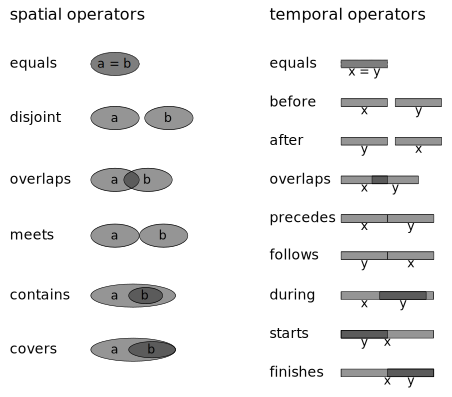
\includegraphics[width=0.6\textwidth]{graphics/basics/spatial_temporal_operators}
  \caption{visualization of spatial and temporal operators}
  {\small alteration of \cite[p. 137-139]{ott2001time}}
  \label{fig:spatial_temporal_operators}
\end{figure}


spatio-temporal queries
  when + where -> what
  when + what -> where
  where + what -> when
  \cite Peuquet 1994

temporal logic
  rules and symbols
  represent time
  reason about time
  temporal operators
  ??? detail?
  \cite Hodkinson and Reynolds 2006

trajectories
  sequence of 2D or 3D locations of an object


concepts of domain
------------------

historical event
  WHAT? significant happening
  WHO? different actors
  WHEN? one point in time
  WHERE? mostly also point in space, sometimes different from area that event affects
  WHY? because

administrative unit
  defined by borders
  hierarchical structure

country borders
  coastlines
  interior
  disputed territories
    situation: n fully recognized countries and m non or partially recognized entities claim sovereignty over 1 territory
    territory is surrounded by disputed border
    question: does this disputed area claim sovereignty?
    \footnote \url{http://www.economist.com/blogs/economist-explains/2014/09/economist-explains-1}
  uncertain borders
    situation: n fully recognized countries commonly agree on a boundary between them, but the border is not clearly defined / fuzzy / uncertain
  states of borders
    planned
    agreed
    demarcated
    provisional
    valid
    vs. disputed

enclaves, exclaves




representation models
---------------------

record objects in time and space

idea: continuous space-time cube
  2 spatial, 1 temporal dimension
  everything changes continuously
  \cite Langran 1992

continuous processes sampled in discrete steps


extension of traditional raster / vector approaches to incorporate time
  organizing dimension: space
  representation: 2D / 3D space (raster: grid, vector: open space)

  Snapshot model
    \cite Armstrong 1988
    1 layer per time point
    layer data
      time point
      fully covered spatial and attribute data
    => full picture at point in time
    (+) simple
    (-) changes not recorded -> can not be retrieved
    (-) no information of status between two time slices
    (-) redundant
    e.g. aerial images
    e.g. social indicators collected by World Bank
    \cite[chapter 2, p. 46]{solana2014spatio}

  Time slices
    discrete slices into time cube
    snap shot time slices
    temporal changes of time slices
    \cite Langran 1993
    \cite[p. 63-64]{ott2001time}

  The grid model
    for raster data: each cell has list of values with time stamps
    change => affected cells get new value with new time stamp
    \cite Langran 1992
    improvement of snapshot model for raster model
    -> only compatible with event-based approach
    (+) no redundancy
    improvement: space-time BLOB
    \cite[p. 14]{zhao11}

  Space-time composite
    decomposition of geometries into least common geometries (LCG) out of which all other geometries can be composited back from
    e.g. Germany (DE), France (FR), Elsaß (EL), before 1919: DE+EL, FR - after 1919: DE, FR+EL
    \cite Langran and Christman 1998
    \cite Worboys 1994
    (+) no redundancy in geometry
    (+) analysis of history of certain areas = LOC is very simple
    (+) supports hierarchical structure of administrative units
    (-) complete structure has to be changed if one event is inserted

  Amendment vector model
    amendment vectors: spatial changes over time
    increment stored on the basis of previous time point
    \cite Langran 1992
    (-) object identity has to be known
    (-) amendment vector only records spatial change => solely attribute change can not be modeled
    \cite[p. 14]{zhao11}

time-based approach
  organizing dimension: time
  representation: time line / temporal vector (1D)

  Simple time-stamping model topology of time
    \cite Langran 1993
    time stamp per object
      date of last property transaction
      period of existence (start - end)
    (+) ability to track changes
    (+) fits perfectly for events with discrete nature
    (-) cumbersome to retrieve
    (-) redundancy for topological geometry (end date of one geometry is start date for another geometry)
    e.g. analysis of spatial diffusion
    e.g. longitudinal analysis (e.g. development of census data throughout the years)
    problem: varying administrative boundaries over time
    solution: aerial interpolation
    \cite[chapter 2, pp. 46-47]{solana2014spatio}

  event-based spatio-temporal data model (ESTDM)
    key elements:
      event list (event = change in state)
        recording only times when change occurs -> relation change <-> time
        time-stamp $t_i$
        spatial or attribute change
        doubly-linked ordered list of events for efficient change tracking in both directions
      base map defining initial world state at $t_0$
      header pointing to current event
    event happens => new record of study area
    keeps track of affected cells and their new value
    (+) efficient change tracking
    (+) efficient inserting of events somewhere inside the list
    -> problem: consistent geometry! => update necessary
    (-) not suitable for representation of continuous gradual change
    (-) model explicitly for raster data, not for vector polygon geometry
    problem: maintaining the integrity of spatial topology as it changes
    (-) model just for tracking spatial changes
    -> extension: separate table per attribute dimension
    \cite{peuquet95}

  object-oriented spatio-temporal data model
    2D geometries + 1D time
    element: spatio-temporal atom
    event-based: new event => new ST atom stacked on top of existing ones
    \cite Worboys 1992

cell tuple-based spatiotemporal data model
  \cite Raza and Kainz 1999

Claramunt and Thériault 1995
Chen and Jiang 2000
Worboys 2005


concepts of time and space
--------------------------

based on geographic events
space: GIS only recognize space that is occupied by objects \label{gis_space_theory}
time: event vs. process
  event
    discrete
    occurrence / outcome with significance
    time point vs. time periods
  process
    continuous
    series of events of one kind leading to a common goal
  \cite Worboys 1998
  event-based HGIS: store only events (discrete, just like spatial objects)
  process-based HGIS: continuous time span of interest
\cite[chapter 2, pp. 47-49]{solana2014spatio}

valid / world time
  time was true in reality
transaction / database time
  time it was stored in the database
\cite Jensen et al. 1993
\cite[p. 69]{ott2001time}

Time Geography
  orthogonal relationship between time and space
  each object can be at one time only at one location
  happenings and events
  \cite Hägerstrand 1970

space-time path / space-time graph

``Geography differs from geometry because in geography, space in indivisibly coupled with time''
(Don Parkes & Nigel Thrift 1980)

version management
------------------

database has to be updates when change occurs
versioning methods
  relation-level versioning
    rollback: new event -> new snapshot
    type of change (added, altered/updated, deleted, restored)
  tuple-level versioning
    store changes with event time
    => time slices can be derived from the information about changes
    (+) less redundancy, less data
    (-) weaker performance on retrieval
  attribute versioning
    -> extension of tuple-level versioning: separation entity <-> attribute
    changes stored in attributes
\cite Langran 1989

international boundary has different states:
  event           old b.    new b.              active
  -               valid     -                   old
  legal document  invalid   -                   old
  new demarcation invalid   draft -> invalid    old
  quality control invalid   valid               new
-> stati: valid, draft, revised, approved = valid
check on consistency_> only one version accessible to public
\cite Wachowicz 1999


spatio-temporal databases
-------------------------
how to store and query spatial and temporal data?

static databases
  no updates, old information overwritten by new information
  -> not suitable for spatio-temporal object management
static rollback approaches
  implementation of relation-level versioning
  change -> copy old data, change elements to new data => complete new time slice
  (+) effective versioning
  (+) fast retrieval of state at time point x
  (-) highly redundant
historical databases
  store valid state at a specific time point (valid time)
  store time slices valid for specific time steps
  or validity of objects between events
  -> changes only made with valid time
temporal databases
  support both valid and transaction time
  retrieval of current state at given time step
  (+) supports retrieval of what was known to the database at given time point
  usage in knowledge and research database
  usage when different sources for same event are used
  -> supports different views on world

implementation using relational databases
separation time and space in database

ER model for temporal objects
  \cite Basogly & Morrison
  example: administrative units
  units change borders and attributes over time
  units valid over certain period of time
  units have ancestors and successors
  -> units gain area from or loose area to one or several other units
  hierarchical structure of units (country -> state -> county -> city -> neighborhood -> ...)
  units can have additional attribute data (e.g. statistics per year)
  \cite Pierau 1998
  \cite[p. 67-68]{ott2001time}

Spatio-Temporal Data Type
  STT
  time not as an attribute of space -> special entity
  spatio-temporal object model (everything is an object)
    separate classes for Space and Time
    -> aggregation to SpatioTemporal class
    each object with temporal and spatial extension (start + end date, full geo)
  operators for time and space
  time in YYY-MM-DD (ISO 8601 standard)
    `NOW' = still existing = no end date
  \cite{raza12}


implementation
--------------

historical R-tree
  assign timestamp t_i -> active objects = [o_1, 0_2, ... , o_n]
  (+) fast handling of timestamp
  (-) redundancy, because of repeating objects

MV3R tree (Tao & Papadios, 2001)
  version copy
  (+) less redundant


spatio-temporal analysis
------------------------

analysis: determine, change, evaluate

multivariate historical-geographical model
  multivariate
    features of a spatial object
    connection between temporal development of features
  geographical model
    location (geometry)
    neighborhood relation (topology)
  historical model
    object at different points in times
\cite[p. 128]{ott2001time}
\cite Kilchenmann 1992

analysis methods
  spatial analysis
  temporal analysis
    time series analysis
    process analysis      (modification modeling + future forecasting)
  attribute analysis
alteration of \cite[p. 128]{ott2001time}

spatial queries
  query of spatial properties and attribute values
  e.g. size of Germany in 1871
thematic queries
  query objects based on certain criteria (spatial and attribute)
  multi-criteria analysis
  e.g. all democratic countries larger than 10.000 km²
statistical analysis
  artithmetic calculation and classification of characteristics of objects
  univariate, multivariate investigation
  e.g. What was the population density in Germany in 1945 compared to 1995
overlay/split
  aggregation and splitting of spatial components based on the layer principle
  e.g. Germany in 1945 gets split up into FRG and GDR by one polyline (inner German border) and one polygon (West Berlin)
geometric-topological operations
  analyze the neighborhood relations between geometric objects
  e.g. is the geometry all countries at time point 1991 strictly connected?
temporal analysis
  using spatial and temporal operators in figure \ref{fig:spatial_temporal_operators}
  e.g. in which year did the largest amount of border changes happen?
\cite[p. 129-140]{ott2001time}

non relevant for thesis:
  interpolation
    Based on the data in the dataset predict values not part of the dataset
    point interpolation
      e.g. temperature at two points, what is the temperature at the place in the middle?
    area interpolation
      e.g. reasonable comparison of fertility rate in Germany in 1939 and 1949
  network function
    network structures -> path search (shortest path, fastest route, TSP)
    network topology


spatio-temporal visualization
-----------------------------

maps are means and products of GIS

scientific visualization vs. information visualization
  tangible objects            abstract concepts
  with inherent form          without inherent form
  e.g. CT scan of human body  e.g. flow of refugees
-> 3D globe: inherent form, direct representation of Earth -> scientific visualization
-> 2D map and time: no inherent form resp. abstract concept
=> information visualization

tasks of visualization
  present (what? where? when? how?)
  analyze (e.g. what is the best? where is the most? when was the first?)
  explore (why?)
\cite Kraak 1999

interactive map enhances human cognition (panning, zooming, changing map layers, time point, data source, ...) and lets him gain knowledge about the domain

maps contain symbols and elements
  ... blaaa ...

traditional paper maps vs. modern digital maps
\begin{table}[ht]
\centering
\begin{tabular}{llp{1em}ll}
    \toprule
    \multicolumn{2}{c}{classical map} & & \multicolumn{2}{c}{modern digital map} \\
    Charaktercharacter & restriction & & character & improvement \\
    \midrule
    static & only discrete point in time & & dynamic & higher sample rate for continuous processes \\
    isolating & only part of geographical space in 2D & & multi-dimensional & multiple levels of detail, possibility for representation of elevation and temporal dimension \\
    selective & only one layer & & inclusive & change layers and perspectives \\
    passive & only sending information & & interactive & direct manipulation and exploration \\
    \bottomrule
\end{tabular}
\caption{Innovation of modern digital maps}
\small{alternation of \cite{karcher} and \cite[p. 145]{ott2001time}}
\label{tab:maps_restrictions}
\end{table}

modern digital maps can show changes in time and space due to their dynamic, multi-dimensional, inclusive and interactive nature.

spatial domain
  2D: map, different projections
  3D: globe

temporal domain
  linear time
    time line
    time series: graph (t,y coordinate system)
    2.5D map: temporal dimension on z axis or on surface
    space-time path
  cyclic time
    time series: polar diagram
    time wheel
  both
    mono-temporal: one layer -> one time point
    multi-temporal: one layer -> multiple time points
\cite[p. 144]{ott2001time}

direct display of time on a map
  choropleth maps
  temporal diagrams
  change indicators

display mechanisms for visualizing temporal change
  change data         additional to base map (diagrams, texts)
  static symbols      thematic map, symbols: dates, routes, developments
  time sequence maps  mono-temporal maps in sequence
  animations          interactive visualization of time and space and attributes
\cite[p. 146-147]{ott2001time}


other approaches
  scatterplot               variation of two variables over time
  parallel coordinate plot  variation of multiple variables over time
  time series graph         variation of one variable over time

visualization in a way that people can understand it
  self-organizing map (SOM) nD variables -> 2D space + 2D color scheme
  \cite Guo et al 2006


HGIS presentations / usage
--------------------------
there is ``not any operational temporal GIS''
\cite[p. 5]{raza12}

  \emph{lifelines}
    showing tracks, routes and meetings or people -> linear, time steps
    historic example: Napoleons Moscow Campaign
    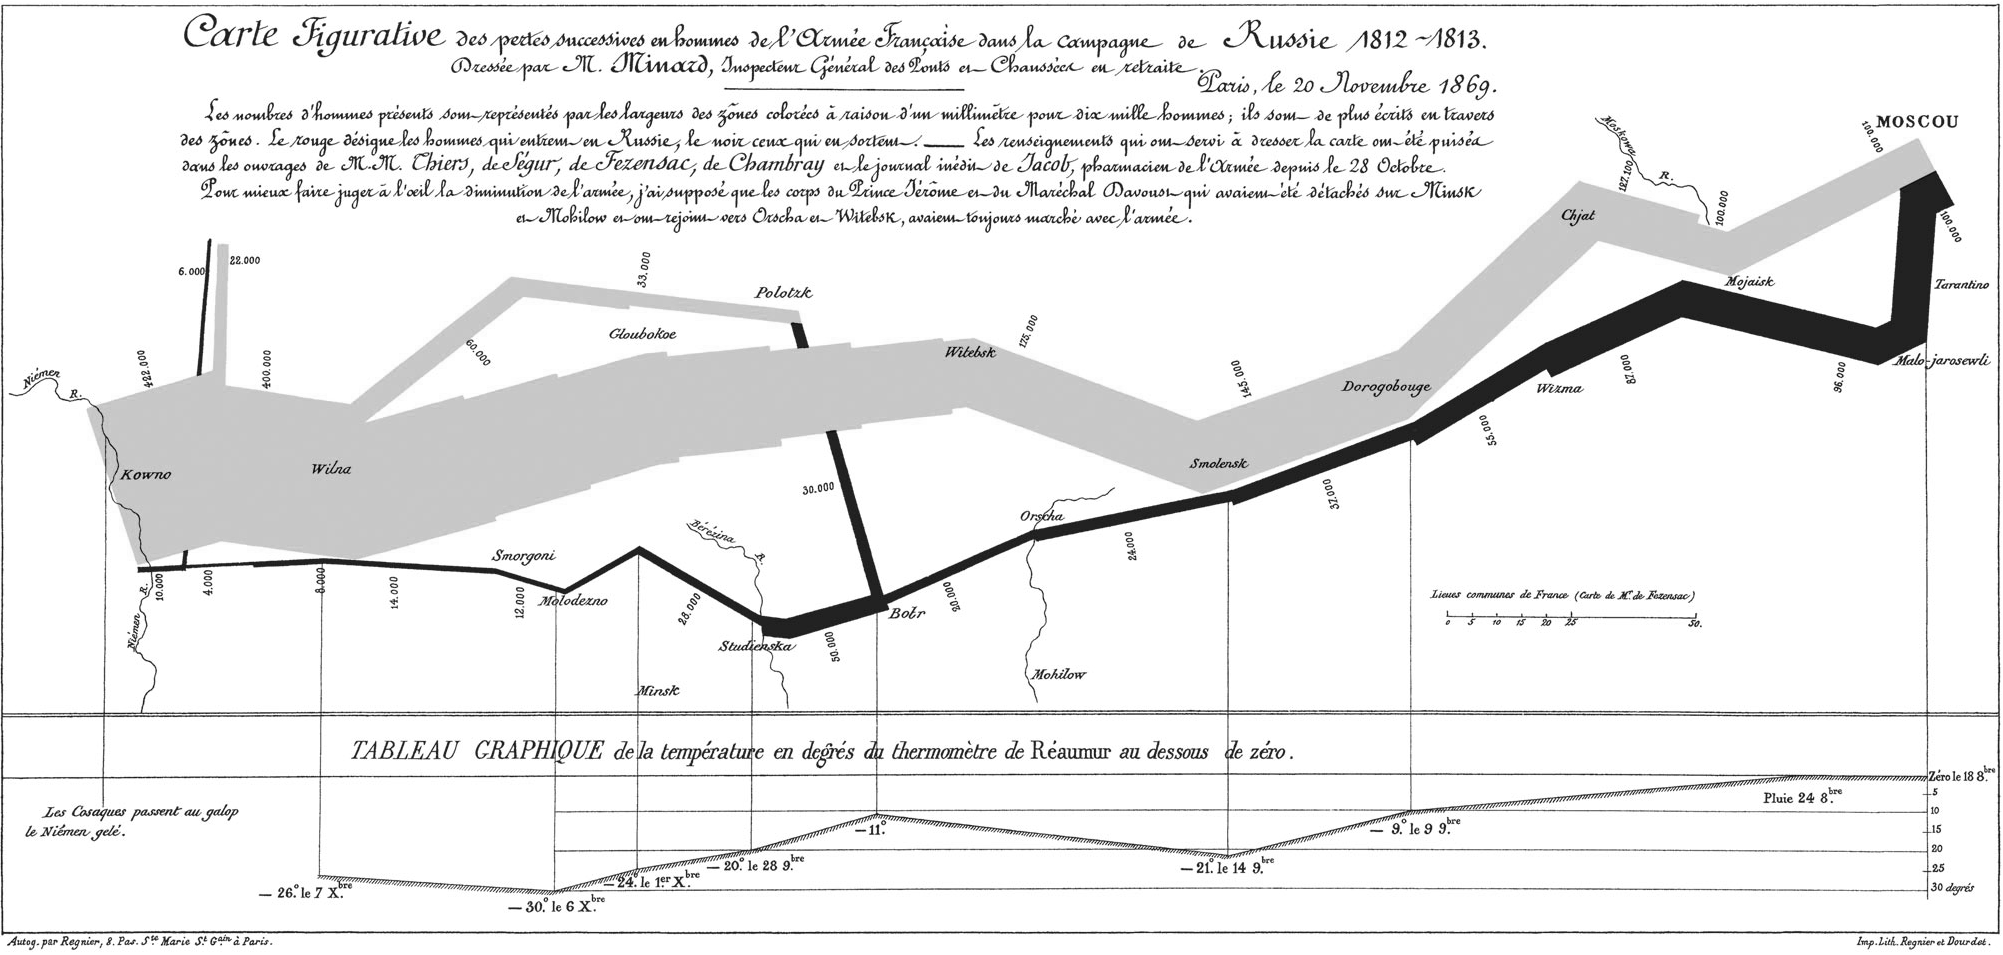
\includegraphics[width=0.8\textwidth]{graphics/napoleon_march_moscow.png}
    \footnote{
      \textit{Minard.png}
      Charles Minard, 1869,
      URL: \url{https://commons.wikimedia.org/wiki/File:Minard.png},
      last access: 03.11.2015,
      Charles Minard's 1869 chart showing the number of men in Napoleon’s 1812 Russian campaign army, their movements, as well as the temperature they encountered on the return path. Lithograph, 62 x 30 cm
    }
    \cite[pp. 188-191]{knowles2008placing}

  reason about historical events
    combine spatial and temporal and attributional information -> overlays
    e.g. Battlefield stories (what was the cause for the victory of party A?)

  mapping historical maps (historical status)
    most part of the work: digitizing and systematizing primary source material into spatial and attribute data (geodata)
    -> georeferencing, semi-automatic feature extraction, manual data entry
    \cite[pp. xvii]{knowles2002past}
    There are several techniques to acquire geodata as a primary source, e.g. through surveying, aerial and satellite imaging using remote sensing and photogrammetry
    \cite[p. 148-149, p. 213-216]{bolstad2008gis}.
    Spatial data from a hardcopy map can be gained by a two-step process that can be seen in figure \ref{fig:hibo}:
    First project the map into the coordinate system of the world by \emph{georeferencing}. The result is that each pixel of the raster graphic is assigned a geographic coordinate from the real world, so the geometry is given a spatial reference. Afterwards acquire the coordinates of the desired features on the map through semi-automatic digitizing
    \cite[p. 133-142]{bolstad2008gis}.

    \begin{figure}[ht]
      \centering
      \begin{subfigure}{0.48\textwidth}
        \centering
        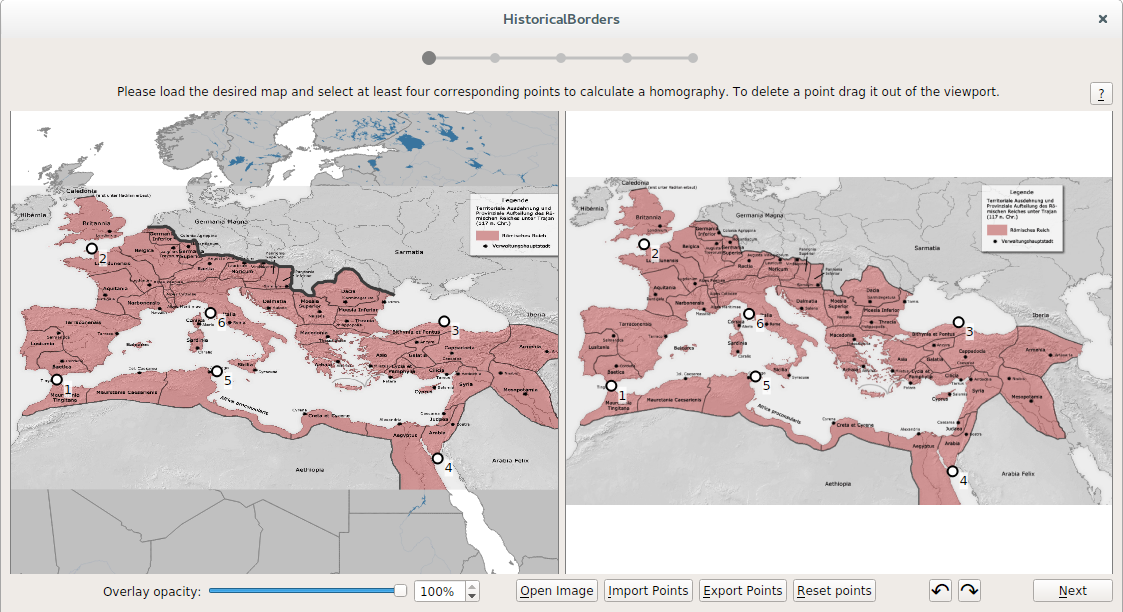
\includegraphics[width=0.95\linewidth]{graphics/hibo1.png}
        \caption{Georeferencing}
      \end{subfigure}
      \begin{subfigure}{0.48\textwidth}
        \centering
        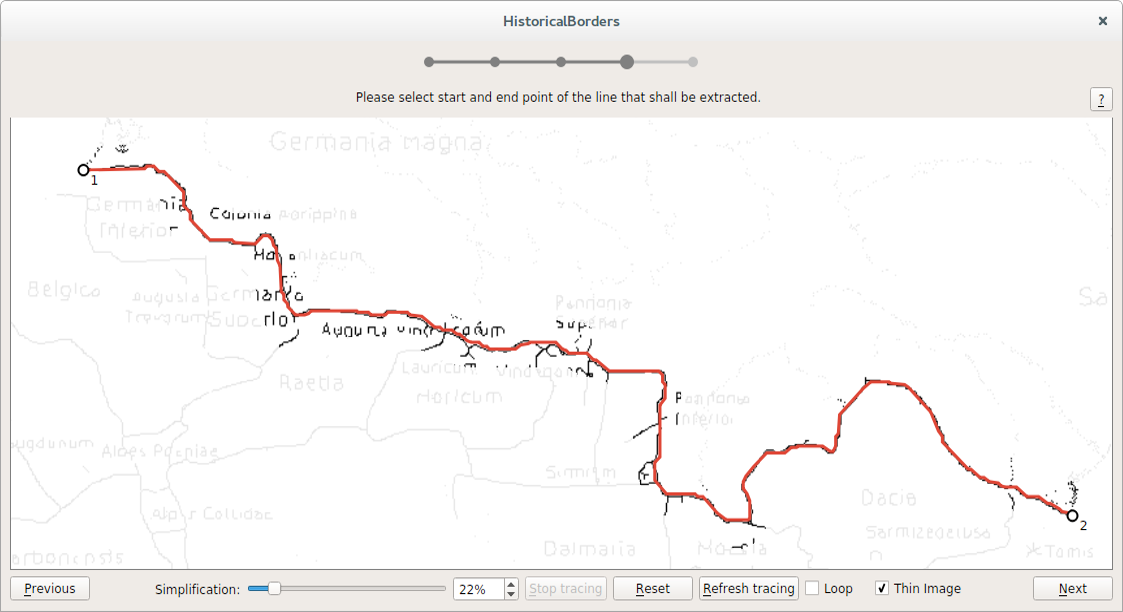
\includegraphics[width=0.95\linewidth]{graphics/hibo2.png}
        \caption{Semi-automatic digitizing}
      \end{subfigure}
      \caption{Semi-automatic extraction of a border from a map of the Roman Empire \protect\footnotemark}
      \label{fig:hibo}
    \end{figure}

    \footnotetext{
      \textit{HiBo - semi-automatic extraction of borders from historical maps},
      Project of: B. Weber, N. K. Dankwa, K. Singh and T. Kashyappan, supervised by: Prof. Volker Rodehorst and Marcus Kossatz, Bauhaus-Universität Weimar, February 2015,
      URL: \url{https://bitbucket.org/bastian_weber/hibo},
      last access: 29.10.2015
    }


HGIS projects
  usage: mostly quantitative research
  -> logical characteristics of information system)

  large collection of research projects
  \cite{knowles2008placing}
  \cite{gregory2014toward}

  ``The Barrington Atlas of the Greek and Roman World''
    gazetteer: name of historic place -> map by map
    \cite{talbert2000barrington}
    \footnote{
      \textit{Ancient World Mapping Center},
      The University of North Carolina,
      URL: \url{http://awmc.unc.edu/},
      last access: 03.11.2015
    }
  solution
    think about how to represent historical knowledge in geographic context
    degree of certainty -> ironically: that has to be exact as well in a database table
    => reason: careful conclusions from historical maps
  problem: tedious manual work
    ~20 hour per map already digitized
    \cite[pp. 145]{knowles2002past}

  show change over time (historical development)
  state-based approach (photography: validity period of geometries)

  ``Great Britain Historical GIS Project'' (GBHGIS)
    \footnote{
      \textit{Great Britain Historical Geographical Information System (GBHGIS)},
      Ian Gregory \& Humphrey R. Southall, University of Portsmouth, since 1994,
      URL: \url{http://www.port.ac.uk/research/gbhgis/},
      last access: 02.11.2015
    }
    idea:
      combine statistical data with territorial units
      => new analytical opportunities
      e.g. analyze net migration in the districts in UK
      -> snapshot model
    problem:
      ``To map and spatially analyze data correctly, quantities must be linked to an accurate representation of the units for which they were collected.''
      administrative units / districts fundamentally changed three times and slightly changed hundreds of times over the last 200 years
      statistical data is gathered per unit
      hardly any info about historical boundaries of districts
      (some by British Ordnance Survey, but not covering everything)
      => results would be disproportional
    \cite[pp. 117-129]{knowles2002past}
    solution: aerial interpolation
      geostatistical interpolation
      discrete data proportional to source polygon (old geometry) -> reaggregate to target polygons (new geometry)
      => prediction
      \cite{aerialInterpolation}

    UK ordnance survey
      * automatic change detection
      \url{https://www.ordnancesurvey.co.uk/education-research/research/automatic-change-detection.html}

  ``National Historical Geographic Information System'' (NHGIS)
    \footnote{
      \textit{Welcome to NHGIS},
      Minnesota Population Center, University of Minnesota,
      since 2007,
      URL: \url{http://www.port.ac.uk/research/gbhgis/},
      last access: 02.11.2015
    }
    idea:
      provide digital boundaries for each census year
      -> estimation of population of any year
    concept:
      composite map: each face represents an area that never changed
      -> composition to regions per year based on compositing information
      dealing with problem of varying administrative borders through aerial interpolation
    interface:
      very scientific a lot of options
      need tutorial to go through the selection
      need to register before downloading something
      get a link to download a file
      have to decompress it
      then load it into your preferred GIS
      -> incredibly frustrating !!!


This application does maps and timelines:

https://www.palantir.com/palantir-gotham/applications/

MAP
The Map application delivers geospatial analytic capabilities. It combines the visualization of geo-located objects on a map with histogram, timeline and time wheel visualizations. A heatmap visualization illuminates the density of interesting objects on the map.

The imagery on the Map is fully pluggable, allowing users to switch between different sources of imagery, integrate private imagery, and create composite imagery sets that combine two or more sources of imagery.

KML and Shapefiles can be imported as independent map layers, and shapes contained in these layers can be used to select and filter objects that lie in a similar region (like a county, census plot, or state). Layers can be colored and labeled according to calculations performed on the data they contain.


Here is a group using the tool to do historical maps: http://envisioninghistory.org/


And here is a program I’m using for my dissertation. I don’t know if it does timelines and maps, but I think it might.

http://www.tableau.com/

Here are some examples of what I’m doing with it: https://public.tableau.com/profile/ammon.shepherd#!/

And my dissertation website just for fun: http://nazitunnels.org



uncertainty
-----------
  -> Managing Vagueness, Uncertainty and Granularity in Spatial Information Systems (VUG)
  %http://www.geos.ed.ac.uk/~gisteac/gis_book_abridged/files/ch13.pdf
  %http://link.springer.com/chapter/10.1007%2F978-3-642-14755-5_1
  %http://support.esri.com/en/knowledgebase/GISDictionary/term/uncertainty
  %http://www.geog.ucsb.edu/~kclarke/G176B/Lecture07.ppt
  -> Karl Grasser (Diss. Santa Barbara)
  -> Fuzzy, Imprecice,
  proabilities vs. possibilities

big problem: why? intention and motivation of author? hard to find out...
voice and perspective
medieval maps: natural landmarks as border points => inaccurate and imprecise
perspective: who is making the map? (illiterates?)
different names:
  US Civil War (North) vs.
  WWI (West) vs. Germanic War (Russia)
  WWII (West) vs. Great Fatherland War (Russia)

accepted uncertainty: date != exact timepoint, only D.M.Y
                      location != exact location, only name of place


step further: temporal GIS to narrative GIS
-------------------------------------------

idea: explain history with spatial narratives
  geographically contextualize events and interactions
  organizing principle: time


\cite[chapter 2, p. 51]{solana2014spatio}

space-time premise by Gaddis 2002
  time and space equal importance
  event     what significantly has happend and by whom? (singularity!)
  process   how something has happened? (event+activity => trigger of process)
  change    driven by process
  spatiotemporal data defines all above three
  \cite Gaddis 2002





% ------------------ MY APPROACH ------------------ %
changed-based approach (historical event -> .. -> geometry changes)
  is there something ?!?
  -> MY APPROACH!
usable User Interface for both navigation and editing
-> problem: all interfaces are trés horrible!

no perfect data model possible, because a model is just an incomplete abstraction of the real world

map for spatial domain (x, y)
timeline for temporal domain (t)
-> 3D system

no transaction time, only valid / event time

space-time composite with lines

\ref{gis_space_theory}
-> the whole earth is 100\% covered by spatial objects (full topology)
  countries, debated territories, unknown land, water
  Newtons concept of absolute space?

ancestors successors
layers of administrative units
open to extension for additional attribute data (e.g. statistics)

geometries must be edited

% ------------------------------------------------- %

requirements
  geographical knowledge
  contextualize / intersect historical sources
  accept imprecision
  prevent illusion of certainty

describe the components of the GIS explicitally
 hardware
 software
 data

 collection
 management
 analysis
 output

% --------------------- CONTEXT --------------------- %
research questions --> HGIS <-- development of system
  historians /                           ME
  geographers
(+) open source, direct manipulation, easy sharing and collaboration
